\rhschapter{Refleksion}
De nævnte emner i dette afsnit er noget gruppen er blevet enige om, og individuelle holdninger er der ikke blevet taget højde for i rapporten.\\
\\
\textbf{Sygdom}\\
Vi har haft lidt sygdom, både en med ondt i ryggen og en med forkølelse. Da vi arbejdede meget på flextid, har det ikke påvirket processen særligt meget.\\
\\
\textbf{Blueprints}\\
Taget lang tid at finde ud af at gøre nogle bestemte ting, men generelt set er det gået godt.\\
\\
\textbf{Rapportskrivning}\\
Det gik godt i starten af projektet, men langsommere da produktet var lavet og der skal skrives om implementeringen og rettes til i rapporten.\\
\\
\textbf{Hjemmearbejde}\\
Det har virket okay, på flextid har vi kunne arbejde når vi bedst var inspireret. Kommunikationen er lidt langsommere end hvis man sidder sammen i skolen.\\
\\
\textbf{UP}\\
Vi har efter bedste evne forsøgt at holde UP-arbejdsgangen og det er lykkedes ganske udmærket.\\
\\
\textbf{Gruppens Samarbejde}\\
Vi har ingen konflikter haft i gruppen. Vi har holdt opsamlingssamtaler et par gange om ugen for at høre hvor langt hver enkelt gruppemedlem var nået med sine opgaver.\\
\\
\textbf{Tidsplanen}\\
Vi har lavet et Gantt-diagram som vi har forsøgt at følge. Det er gået godt med de fleste af opgaverne på tidsplanen, men den sidste rapport skrivnings periode er skredet lidt ind over julen, hvor vi gerne ville have haft den færdig inden jul.\\

\begin{figure}
	\begin{center}
		\caption{Gantt Chart efter udvikling.}
		\label{dia:ganttpost}
		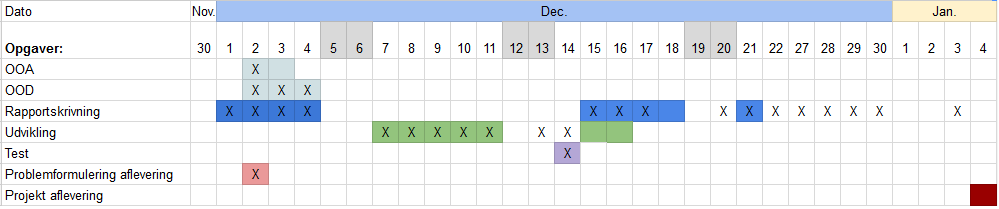
\includegraphics[width=1\linewidth]{pictures/up/ganttpost}
	\end{center}
\end{figure}

